\section{Introduction}

High-fidelity simulations of physical systems can be expensive when repeated predictions are required across many parameter settings. Reduced-order models (ROMs) provide compact surrogates by representing the physical state with a small number of coordinates and evolving those coordinates in time. Their construction becomes more difficult when changing a parameter also changes the type of behavior that must be predicted. In incompressible flows, for example, varying the Reynolds number can lead from relaxation toward a steady state to oscillatory growth and sustained periodic motion. A useful predictive model must capture these behaviors while evolving autonomously: after initialization from a short history, it must use its own predictions rather than future reference states.

This setting presents two related but distinct challenges. The first concerns representation: spatial structures that are important in one regime may differ from those required in another, making a single low-dimensional basis less effective across the full parameter range. The second concerns dynamics: the reduced evolution law must describe relaxation, instability growth, and nonlinear oscillation. Increasing model capacity does not directly resolve a mismatch in the reduced representation, while improving the representation alone does not ensure accurate recursive prediction. These observations motivate adapting the local representation and the local dynamics separately, while providing a consistent way to assemble their predictions.

Projection-based ROMs provide an explicit reduced representation and reduced dynamics, commonly through proper orthogonal decomposition (POD) and
Galerkin projection \citep{sirovich1987,berkooz1993,benner2015}. Truncation, however, removes interactions that can still influence the retained coordinates, producing closure errors that degrade long-horizon prediction \citep{amsallem2012}. Data-driven reduced models offer greater flexibility in approximating nonlinear dynamics, but low one-step error does not guarantee accurate autonomous rollout \citep{vlachas2018,duraisamy2019,brunton2020}. Hybrid ROMs combine physics-based reduced models with learned corrections or learned reduced representations, retaining physical structure while increasing approximation flexibility
\citep{dar2023,lee2020,fresca2022,geelen2023}. A complementary strategy localizes the reduced representation, using multiple subspaces, clusters, or manifolds for different portions of the solution set \citep{kaiser2014,li2021cluster,diaz2024}. These directions address complementary aspects of the broad-parameter problem: hybrid modeling improves the fidelity of the reduced dynamics, whereas localization adapts the reduced representation to regime-dependent structure.

Localization, however, creates an assembly problem. Independently constructed local ROMs generally have different mean fields, bases, scalings, and reduced operators, so their coefficient vectors are not componentwise comparable without an explicit alignment or change of basis. This does not preclude coordinate-transfer methods; it motivates an alternative based on reconstructed outputs. Mixture-of-experts (MoE) architectures provide a framework for conditional specialization \citep{jacobs1991,jordan1994,shazeer2017,fedus2022}, but many formulations route predictors within a shared representation. We instead distinguish dynamical specialization within each chart from the selection and assembly of complete local ROMs across charts.


To address this gap, we introduce the Regime-Adaptive Localized Mixture-of-Experts Reduced-Order Model (RAL-MoE-ROM), a two-level hierarchy that separates within-regime dynamical specialization from cross-regime model selection and assembly. The parameter domain is covered by overlapping regime-local parameter regions, each equipped with an independent reduced chart and a complete autonomous specialist. Within each specialist, the projected ROM backbone is augmented by a structured sparse MoE correction for unresolved reduced dynamics. Each specialist undergoes closed-loop rollout training, so that its learned correction is optimized under the recursive inputs encountered at inference. At the second level, an outer parameter-only regime router (E2) assigns a trajectory-level preference over local specialists. When two adjacent specialists are both applicable, a learned Top-2 convex fusion (T2-C) uses recent physical history to refine their relative weight. The selected specialists encode the same physical history in their own coordinates and evolve independently. Their predictions are combined only after reconstruction in the common physical space, and the fused output is not fed back into either local trajectory.


\paragraph{Scope.}
We study fixed-parameter prediction windows on prescribed, overlapping regime-local charts. Regime adaptation refers to learned selection and output assembly within this coverage, not unsupervised discovery of bifurcation boundaries. Both the outer preference and the fusion weight remain fixed within a window; the method does not switch charts online along that window. A local specialist may nevertheless represent transient growth and saturation. Initialization requires a short velocity--pressure history: only E2, not the complete prediction pipeline, is parameter-only.

Our contributions are threefold:
\begin{itemize}
    \item \textbf{A two-level hierarchical MoE for reduced dynamics.}
    The first level performs sparse conditional correction within each
    regime-local ROM, while the second selects or combines complete local
    ROMs across regimes. This separates within-regime dynamical
    specialization from cross-regime model selection.

    \item \textbf{Structured autonomous regime-local specialists.}
    Each specialist retains an explicit projected ROM backbone and augments
    it with sparsely routed structured corrections trained under closed-loop
    rollout. The correction experts combine nonlinear, linear, and low-rank
    quadratic responses, providing flexible unresolved dynamics without
    replacing the underlying projected model.

    \item \textbf{Physical-space assembly across independent local ROMs.}
    Adjacent specialists retain independent coordinates and autonomous
    trajectories. T2-C combines only their reconstructed physical fields
    through a history-conditioned convex weight, avoiding direct
    interpolation of reduced states or operators.
\end{itemize}

\par
\begin{figure}[t]
    \centering
    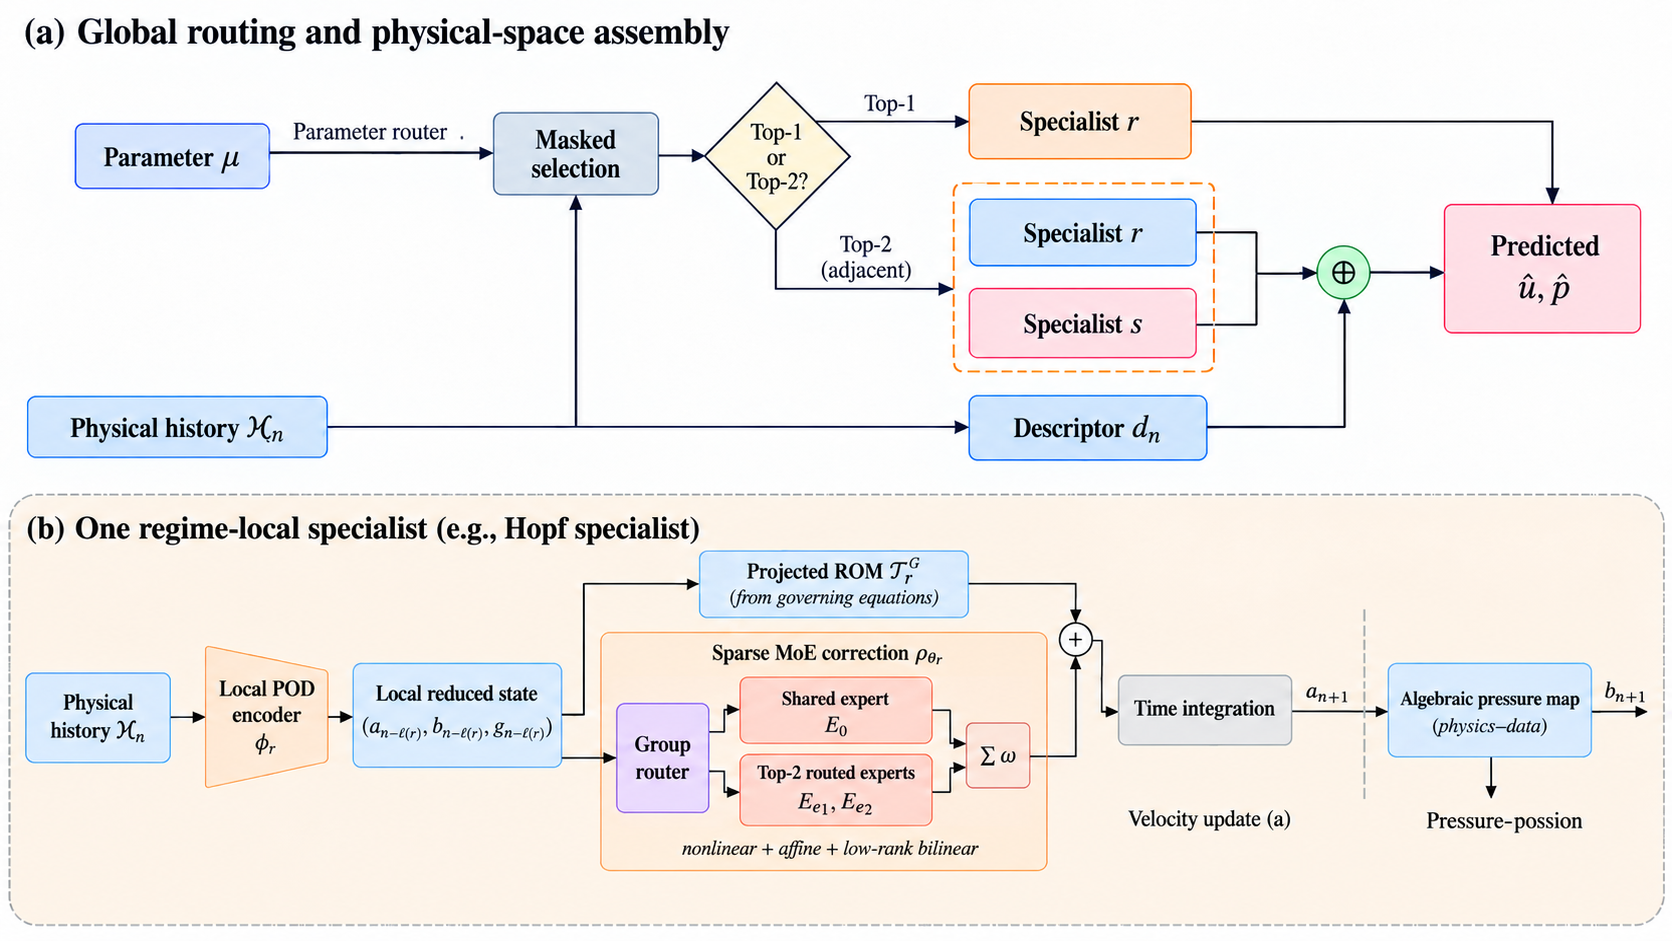
\includegraphics[width=\linewidth]{figures/ral_moe_rom_overview_user_20260908.png}
    \caption{
    Overview of RAL-MoE-ROM.
    (a) A parameter-only outer router selects one regime-local specialist or an adjacent pair. Selected specialists encode the same physical history in their native coordinates, evolve independently, and are combined only after reconstruction; recent physical history conditions the Top-2 fusion but not the outer router. (b) Each specialist augments the projected Galerkin backbone with a structured sparse MoE correction, while pressure is reconstructed algebraically. Flow thumbnails are schematic.
}
    \label{fig:ral_overview}
\end{figure}
\par
